\documentclass[11pt,a4paper]{article}
\usepackage{graphicx}
\usepackage{epstopdf}
\usepackage{amssymb}
\begin{document}
\title{COMP21111 Revision Notes}
\maketitle
\tableofcontents
\newpage
\setlength{\parindent}{0pt}
\section{Introduction}
Just a short introduction to say that I've written these notes to the best of my understanding of the syllabus, I hope they are right, but if you spot any errors, please tell me (you can email me at Isona7@hotmail.co.uk or message me on Facebook where I am Izzy Whistlecroft)!

These are notes for Logic \& Modelling, the exam for 2014 is on the 23rd of January, at 2PM, and is worth 80\% of the marks. Good luck!

PS: I've not written any notes for Lecture 1, as it seems to be mostly fluff, the "good stuff" starts at Lecture 2.
\section{Lecture 2}
\subsection{Propositional Logic Syntax}
Every variable is a \emph{formula}, also known as an \emph{Atomic Formula} or an \emph{Atom}.

$\top$  and  $\bot$ are formulas.

If \emph{A} is a formula, then \emph{$\neg$A} is a formula.

$\top$, $\bot$, $\vee$, $\wedge$, $\neg$, $\rightarrow$, $\leftrightarrow$ are \emph{connectives}.

\subsection{Subformulas}
Formulas $A_1, .... ,A_n$ are immediate subformulas of $(A_1 \wedge ... \wedge A_n)$ and $(A_1 \vee ... \vee A_n)$.

Formula A is an immediate subformula of $\neg$A.

Formulas A and B are immediate subformulas of (A $\rightarrow$ B) and (A $\leftrightarrow$ B).

Every formulas is a subformula of itself.

If A is a subformula of B and B is a subformula of C, A is a subformula of C.

\subsection{Connective Table}

\begin{tabular}{l | c | r}
Connective & Name & Precedence \\
\hline
$\top$ & verum \\
$\bot$ & falsum \\
$\neg$ & negation & 5 \\
$\wedge$ & conjunction & 4 \\
$\vee$ & disjunction & 3 \\
$\rightarrow$ & implication & 2 \\
$\leftrightarrow$ & equivalence & 1 \\
\end{tabular}

\subsection{Parsing}

Parsing $\neg A \wedge B \rightarrow C \vee D \leftrightarrow E$:

\vspace{5pt}
Inside-Out (starting with the highest precedence connectives):

$(\neg A) \wedge B \rightarrow C \vee D \leftrightarrow E$

$((\neg A) \wedge B) \rightarrow C \vee D \leftrightarrow E$

$((\neg A) \wedge B) \rightarrow (C \vee D) \leftrightarrow E$

$(((\neg A) \wedge B) \rightarrow (C \vee D)) \leftrightarrow E$

\vspace{5pt}
Outside-In (starting with lowest precedence connectives):

$(\neg A \wedge B \rightarrow C \vee D) \leftrightarrow E$

$((\neg A \wedge B) \rightarrow (C \vee D)) \leftrightarrow E$

$(((\neg A) \wedge B) \rightarrow (C \vee D)) \leftrightarrow E$

\vspace{5pt}
It doesn't really matter what order you insert the brackets!

\subsection{Operation Tables}

\begin{tabular}{l | c r}
$\wedge$ & 1 & 0 \\
\hline
1 & 1 & 0 \\
0 & 0 & 0 \\
\end{tabular}
\hspace{5pt}
\begin{tabular}{l | c r}
$\vee$ & 1 & 0 \\
\hline
1 & 1 & 1 \\
0 & 1 & 0 \\
\end{tabular}
\hspace{5pt}
\begin{tabular}{l | c}
$\neg$ \\
\hline
1 & 0 \\
0 & 1 \\
\end{tabular}

\vspace{10pt}
\begin{tabular}{l | c r}
$\rightarrow$ & 1 & 0 \\
\hline
1 & 1 & 0 \\
0 & 1 & 1 \\
\end{tabular}
\hspace{5pt}
\begin{tabular}{l | c r}
$\leftrightarrow$ & 1 & 0 \\
\hline
1 & 1 & 0 \\
0 & 0 & 1 \\
\end{tabular}

\subsection{Interpretations and Models}

We can assign values to boolean variables.
An interpretation is a set of such assignments, also known as truth assignments.

If I(A) = 1, we say that that I is a model of A.

If I(A) = 0, then we say that A is false in I.

A is satisfiable if some interpretation satisfies it.

A is valid (a tautology) if it is true in every interpretation.

A is invalid if it isn't satisfied by any interpretation.

Two formulas are equivalent if they have the same models.

\subsection{Evaluating a Formula}

Evaluating the formula:

$(p \rightarrow q) \wedge (p \wedge q \rightarrow r) \rightarrow (p \rightarrow r)$

$\{ p \mapsto 1, q \mapsto 0, r \mapsto 1 \}$
\vspace{5pt}

\begin{tabular}{l | c}
formula & value \\
\hline
$(p \rightarrow q) \wedge (p \wedge q \rightarrow r) \rightarrow (p \rightarrow r)$ & 1 \\
\hphantom{$(p \rightarrow q) \wedge (p \wedge q \rightarrow r) \rightarrow ($}$p \rightarrow r$ & 1 \\
$(p \rightarrow q) \wedge (p \wedge q \rightarrow r)$ & 0 \\
\hphantom{$(p \rightarrow q) \wedge ($}$p \wedge q \rightarrow r$ & 1 \\
\hphantom{$($}$p \rightarrow q$ & 0 \\
\hphantom{$(p \rightarrow q) \wedge ($}$p \wedge q$ & 0 \\
\hline
\hphantom{$($}$p$\hphantom{$ \rightarrow q) \wedge ($}\hspace{2pt}$p$\hphantom{$ \wedge q \rightarrow r) \rightarrow ($}\hspace{5pt}$p$ & 1 \\
\hphantom{$(p \rightarrow $}$q$\hphantom{$) \wedge (p \wedge $}\hspace{8pt}$q$ & 0 \\
\hphantom{$(p \rightarrow q) \wedge (p \wedge q \rightarrow $}$r$\hphantom{$) \rightarrow (p \rightarrow $}\hspace{8pt}$r$ & 1
\end{tabular}
\vspace{5pt}

The formula is true in this interpretation.

\newpage
\section{Lecture 3}
\subsection{Rewrite Rules}

$\top \wedge ... \wedge \top \Rightarrow \top$

$\bot \wedge A_1 \wedge ... \wedge A_n \Rightarrow \bot$

\hrulefill

$\top \vee A_1 \vee ... \vee A_n \Rightarrow \top$

$\bot \vee ... \vee \bot \Rightarrow \bot$

\hrulefill

$\neg \top \Rightarrow \bot$

$\neg \bot \Rightarrow \top$

\hrulefill

$A \rightarrow \top \Rightarrow \top$

$\bot \rightarrow A \Rightarrow \top$

$\top \rightarrow \bot \Rightarrow \bot$

\hrulefill

$\top \leftrightarrow \top \Rightarrow \top$

$\top \leftrightarrow \bot \Rightarrow \bot$

$\bot \leftrightarrow \top \Rightarrow \bot$

$\bot \leftrightarrow \bot \Rightarrow \top$

\subsection{Evaluating a formula}

The formula

$(p \rightarrow q) \wedge (p \wedge q \rightarrow r) \rightarrow (p \rightarrow r)$

with the evaluation
${p \mapsto 1, q \mapsto 0, r \mapsto 1}$

is equivalent to (having replaced $p$ with $\top$, $q$ with $\bot$ and $r$ with $\top$):

$(\top \rightarrow \bot) \wedge (\top \wedge \bot \rightarrow \top) \rightarrow (\top \rightarrow \top)$

\vspace{5pt}
Applying rewrite rules:

$(\top \rightarrow \bot) \wedge (\top \wedge \bot \rightarrow \top) \rightarrow (\top \rightarrow \top)$

$\bot \wedge (\top \wedge \bot \rightarrow \top) \rightarrow (\top \rightarrow \top)$

$\bot \wedge (\bot \rightarrow \top) \rightarrow (\top \rightarrow \top)$

$\bot \wedge \top \rightarrow (\top \rightarrow \top)$

$\bot \rightarrow (\top \rightarrow \top)$

$\bot \rightarrow \top$

$\top$

\vspace{5pt} The result will be the same, whatever order you rewrite in!

\section{Lecture 4}

\subsection{Compact Truth Table}

\begin{tabular}{l | c | c | c | c}
formula & I1 & I2 & I3 & I4\\
\hline
$(p \rightarrow q) \wedge (p \wedge q \rightarrow r) \rightarrow (p \rightarrow r)$ & 1 & 1 & 1 & 1\\
\hphantom{$(p \rightarrow q) \wedge (p \wedge q \rightarrow r) \rightarrow ($}$p \rightarrow r$ & 1 & 1 & 0 & 0\\
$(p \rightarrow q) \wedge (p \wedge q \rightarrow r)$ & 1 & & 0 & 0\\
\hphantom{$(p \rightarrow q) \wedge ($}$p \wedge q \rightarrow r$ & 1 & 1 & 1 & 0\\
\hphantom{$($}$p \rightarrow q$ & 1 & & 0 & 1\\
\hphantom{$(p \rightarrow q) \wedge ($}$p \wedge q$ & 0 & & 0 & 1\\
\hline
\hphantom{$($}$p$\hphantom{$ \rightarrow q) \wedge ($}\hspace{2pt}$p$\hphantom{$ \wedge q \rightarrow r) \rightarrow ($}\hspace{5pt}$p$ & 0 & 1 & 1 & 1\\
\hphantom{$(p \rightarrow $}$q$\hphantom{$) \wedge (p \wedge $}\hspace{8pt}$q$ & & & 0 & 1\\
\hphantom{$(p \rightarrow q) \wedge (p \wedge q \rightarrow $}$r$\hphantom{$) \rightarrow (p \rightarrow $}\hspace{8pt}$r$ & & 1 & 0 & 0
\end{tabular}

\vspace{5pt} This formula is valid!

The order of variables affects the size but NOT the result!

\subsection{Simplification Rules for $\top$}

$\neg \top \Rightarrow \bot$

$\top \wedge A_1 \wedge ... \wedge A_n \Rightarrow A_1 \wedge ... \wedge A_n$

$\top \vee A_1 \vee ... \vee A_n \Rightarrow \top$

$A \rightarrow \top \Rightarrow \top$

$\top \rightarrow A \Rightarrow A$

$A \leftrightarrow \top \Rightarrow A$

\subsection{Simplification Rules for $\bot$}

$\neg \bot \Rightarrow \top$

$\bot \wedge A_1 \wedge ... \wedge A_n \Rightarrow \bot$

$\bot \vee A_1 \vee ... \vee A_n \Rightarrow A_1 \vee ... \vee A_n$

$A \rightarrow \bot \Rightarrow \neg A$

$\bot \rightarrow A \Rightarrow \top$

$A \leftrightarrow \bot \Rightarrow \neg A$

$\bot \leftrightarrow A \Rightarrow \neg A$

\subsection{Splitting Example}

The idea of splitting is that at each step, you make a branch on a variable, and replace it with $\top$ or $\bot$ (depending on what the variable is on that branch).
Then, apply the simplification rules until it cannot be simplified any more.
Continue doing this until all branches end in $\top$ or $\bot$.

An example of splitting on the formula $(p \rightarrow q) \wedge (p \wedge q \rightarrow r) \rightarrow (p \rightarrow r)$:

\centerline{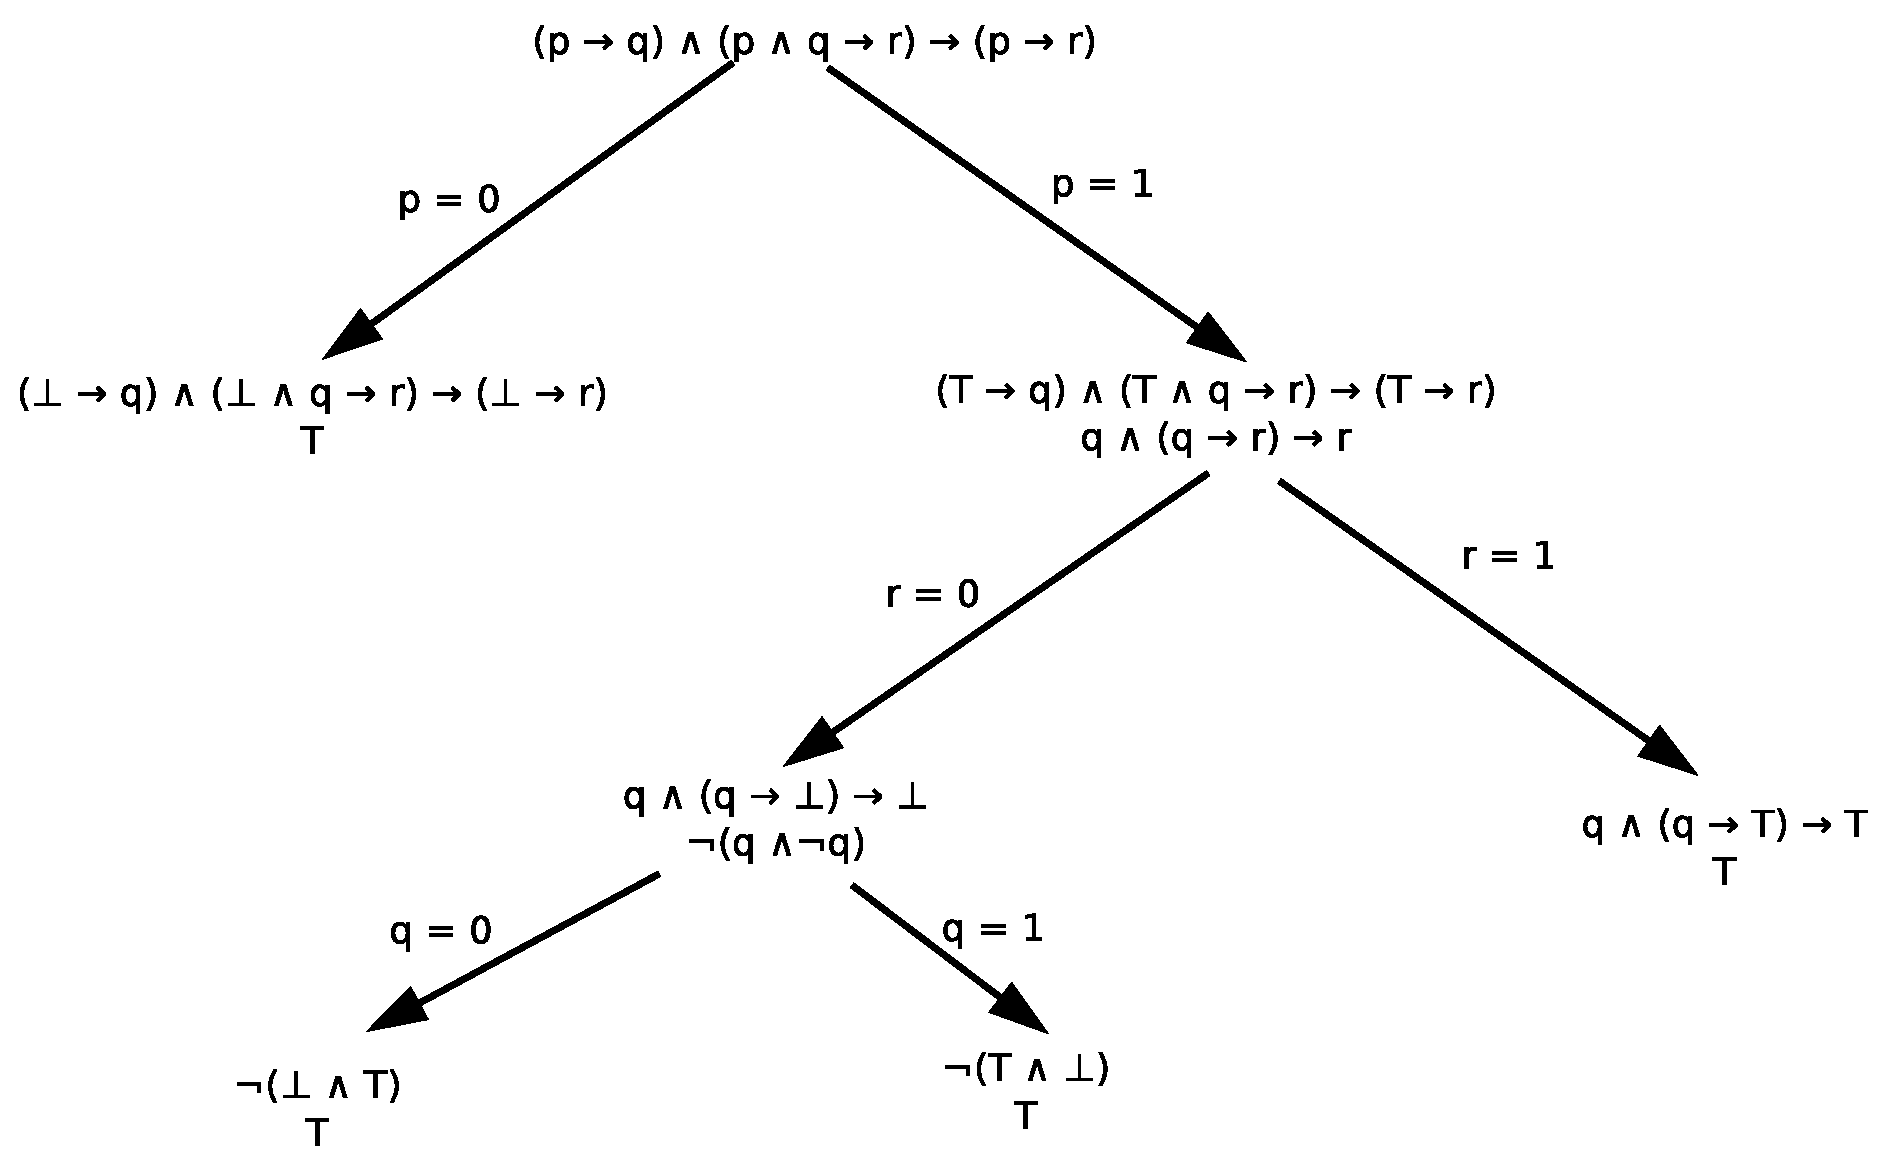
\includegraphics[width=1.00\textwidth]{SplittingExample.eps}}

\subsection{Parse Trees}
An example of a parse tree for the formula $(p \rightarrow q) \wedge (p \wedge q \rightarrow r) \rightarrow (p \rightarrow r)$:

\centerline{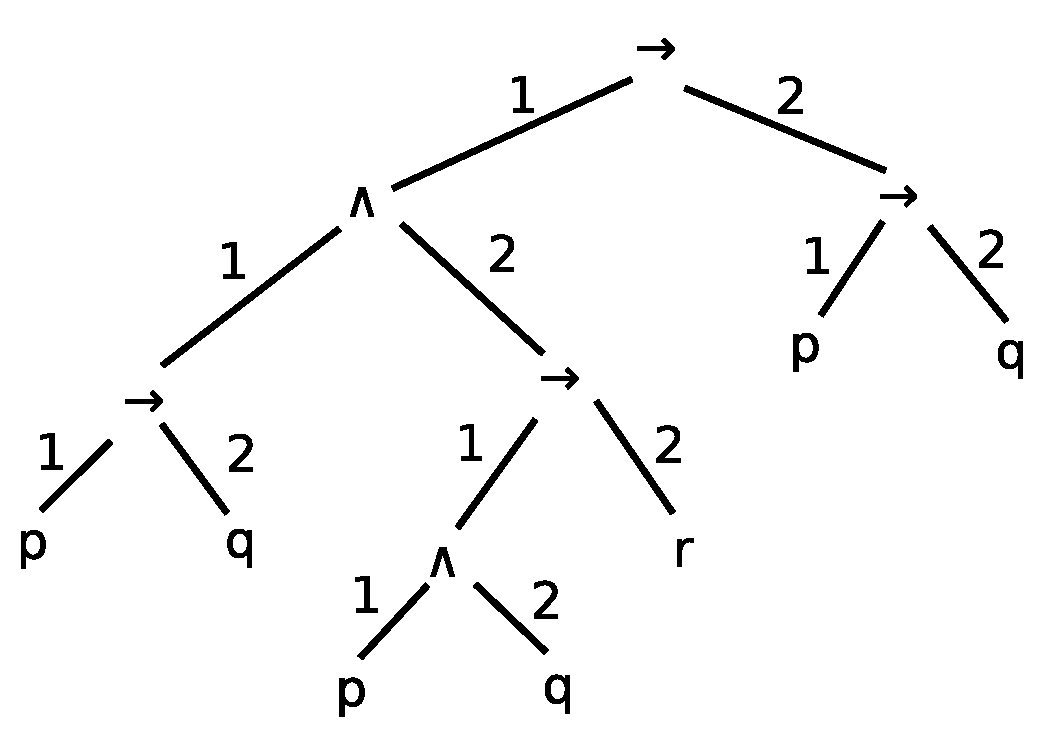
\includegraphics[width=0.5\textwidth]{ParseTreeExample.eps}}

Positions are given by a series of non-negative numbers separated by periods.

A few examples of locations:

The subformula at position 1.2.1 is: $p \wedge q$

The subformula at position 1 is: $(p \rightarrow q) \wedge (p \wedge q \rightarrow r)$

The subformula at position 1.1.2 is: $q$

\subsection{Polarity}

An example showing the polarity of the formula:

$\neg((p \rightarrow q) \wedge (p \wedge q \rightarrow r) \rightarrow (p \leftrightarrow (r \rightarrow q)))$

\centerline{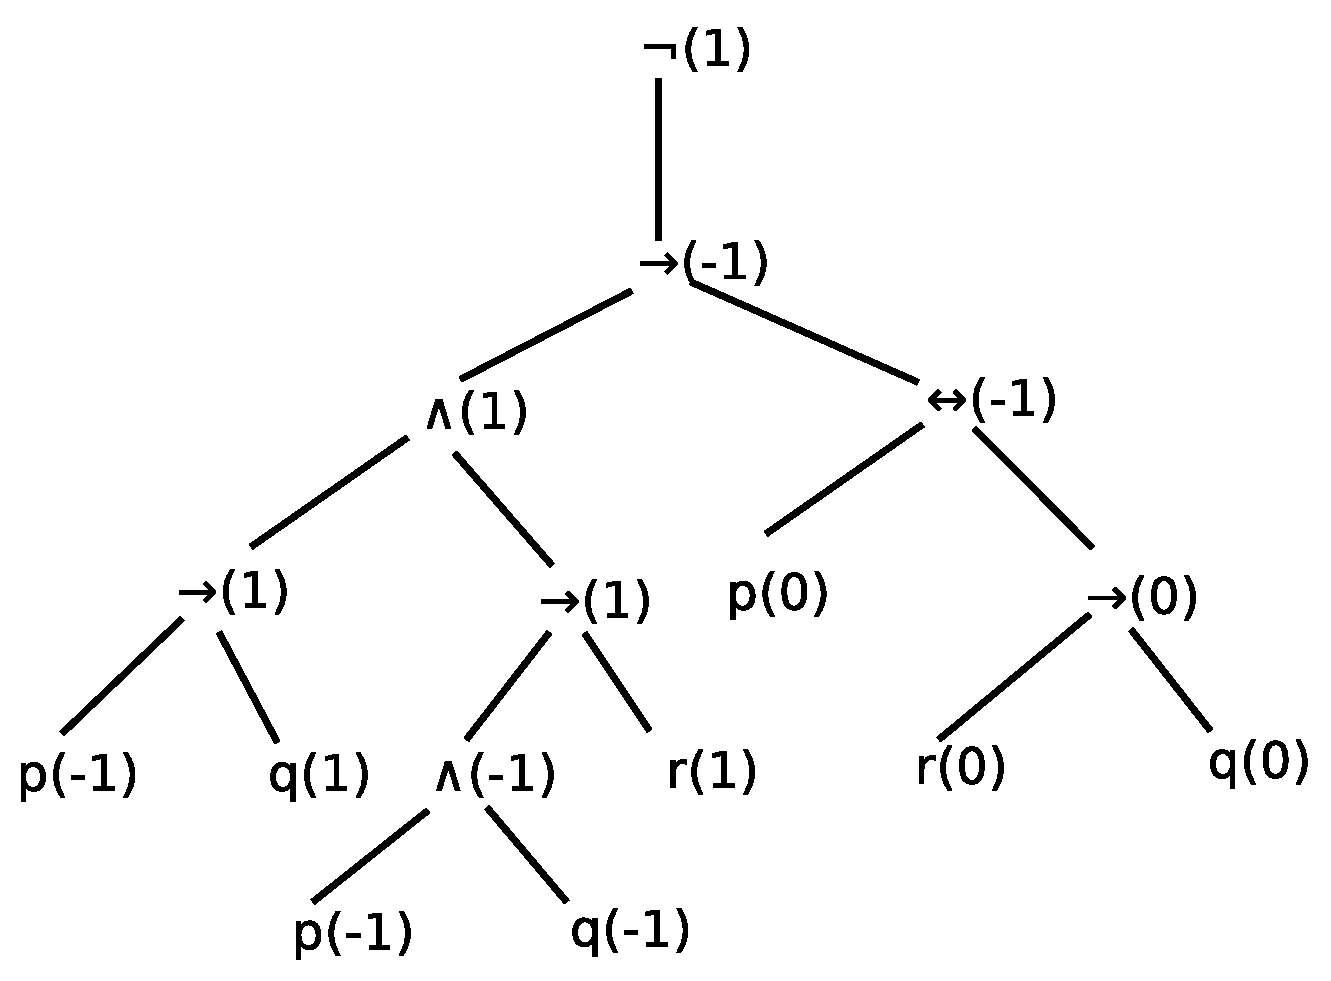
\includegraphics[width=0.75\textwidth]{PolarityExample.eps}}

The polarity of the top node in a parse tree is 1.

The polarity of the node below a $\neg$ is reversed (1 becomes -1, -1 becomes 1).

The polarity of the node to the left of a $\rightarrow$ is reversed, however, the node to the right remains the same (this is because $a \rightarrow b$ can be simplified to $\neg a \vee b$.

All nodes below a $\leftrightarrow$ have polarity 0.

\subsection{Pure Variables}

If all occurences of a variable in a formula are positive, then the formula is only satisfiable if that variable is true.
Likewise, if all occurences are negative, then the formula is only satisfiable if that variable is false.

This means, when checking for satisfiability, pure variables will be replaced with either $\top$ (when polarity is always positive) or $\bot$ (when polarity is always negative).

In the formula $\neg((p \rightarrow q) \wedge (p \wedge q \rightarrow r) \rightarrow (\neg p \rightarrow r))$, $p$ is always negative (trust me on this!).

Due to P being always negative, we can replace $p$ by $\bot$:

$\neg((\bot \rightarrow q) \wedge (\bot \wedge q \rightarrow r) \rightarrow (\top \rightarrow r))$

$\neg(\top \wedge (\bot \wedge q \rightarrow r) \rightarrow (\top \rightarrow r))$

$\neg(\top \wedge (\bot \rightarrow r) \rightarrow (\top \rightarrow r))$

$\neg(\top \wedge \top \rightarrow (\top \rightarrow r))$

$\neg(\top \rightarrow r)$

$\neg r$

Now r is pure (always negative) so we can replace it by $\bot$.

$\neg \bot$

$\top$

\section{Lecture 5}

\subsection{Literals and Clauses}

A literal is an atom or its negation eg $p$ and $\neg p$.

A clause is a disjunction of literals eg $p \vee q \vee \neg r \vee s$.

The empty clause is denoted by $\Box$ and is always false and occurs when there are no literals.

A horn clause is a clause with at most one positive literal.

\subsection{CNF}

A formula is in conjunctive normal form when it is "either $\top$ or $\bot$ or a conjunction of disjunctions or literals".

This means that it will be a formula made only of literals and brackets containing only literals separated by $\vee$, connected by $\wedge$.

Examples:

Correct CNF: 

$p \wedge \neg s \wedge t \wedge (u \vee \neg w \vee x)$

\vspace{5pt}
Not in CNF (there is a $\neg$ outside brackets: 

$\neg(p \vee \neg s \vee t) \wedge u \wedge w$

\vspace{5pt}
Also not in CNF(Bracket in bracket and $\rightarrow$ is not allowed!):

$(p \vee (\neg s \rightarrow t)) \wedge u \wedge w$

\vspace{5pt}
Also not CNF (there are $\vee$ outside of brackets): 

$p \vee \neg s \wedge u \vee w$

The last one in CNF (note the added brackets): 

$(p \vee \neg s) \wedge (u \vee w)$

\subsection{CNF Transformation Rules}

$A \leftrightarrow B \Rightarrow (\neg A \vee B) \wedge (\neg B \vee A)$

$A \rightarrow B \Rightarrow \neg A \vee B$

$\neg(A \wedge B) \Rightarrow \neg A \vee \neg B$ (De Morgan's Law)

$\neg(A \vee B) \Rightarrow \neg A \wedge \neg B$ (Also De Morgan's Law)

$\neg \neg A \Rightarrow A$

$(A_1 \wedge ... \wedge A_m) \vee B_1 \vee ... \vee B_n \Rightarrow (A_1 \vee B_1 \vee ... \vee B_n) \wedge ... \wedge (A_m \vee B_1 \vee ... \vee B_n)$

\subsection{Problems with CNF}

The problem with CNF, is that it may be exponential in size, particularly when $\rightarrow$ and $\leftrightarrow$ are involved.

The solution to this is to introduce definitions/naming.

This involves taking a subformula A, introducing a new name, n for it and then making a statement to say that they are equivalent.

For example:

$p_1 \leftrightarrow (p_2 \leftrightarrow (p_3 \leftrightarrow (p_4 \leftrightarrow (p_5 \leftrightarrow p6))))$

$n \leftrightarrow (p_5 \leftrightarrow p_6)$

Here, a new name n has been introduced for the subformula $p_5 \leftrightarrow p_6$, we can now replace all occurences of this subformula with n
(while still including the definition of n):

$p_1 \leftrightarrow (p_2 \leftrightarrow (p_3 \leftrightarrow (p_4 \leftrightarrow n)))$

$n \leftrightarrow (p_5 \leftrightarrow p_6)$

\section{Lecture 6}

\subsection{Clausal Form}

A clausal form for a formula is a set of clauses which have the same models as the original formula. Clausal form is largely produced by using the naming strategy mentioned in the last section.

The benefit of using Clausal Form over CNF is that clausal form can be produced extremely quickly, while CNF is prone to becoming exponential in size.

\subsection{Clausal Form Transformation}

This algorithm can produce a clausal form of a given formula. The definition of a clausal form is given that as:

If the formula A has the form: $C_1 \wedge ... \wedge C_n$ where each $C_i$ is a clause and there is more than one clause,
the clausal form S of A, has the form $S = \{C_1, ..., C_n\}$.

As with most examples, I have taken this from the slides, but will explain it in more detail below.

\begin{tabular}{c | l | l | l}
& subformula & definition & clauses \\
\hline
& & & $n_1$ \\
\hline
%n1
$n_1$ & $\neg((p \rightarrow q) \wedge (p \wedge q \rightarrow r) \rightarrow (p \rightarrow r))$ & $n_1 \leftrightarrow \neg n_2$ & $\neg n_1 \vee \neg n_2$ \\
&&& $n_1 \vee n_2$ \\
\hline
%n2
$n_2$ & \hphantom{$\neg($}$(p \rightarrow q) \wedge (p \wedge q \rightarrow r) \rightarrow (p \rightarrow r)$ & $n_2 \leftrightarrow (n_3 \rightarrow n_7)$ & $\neg n_2 \vee \neg n_3 \vee n_7$ \\
&&& $n_3 \vee n_2$ \\
&&& $\neg n_7 \vee n_2$ \\
\hline
%n3
$n_3$ & \hphantom{$\neg($}$(p \rightarrow q) \wedge (p \wedge q \rightarrow r)$ & $n_3 \leftrightarrow (n_4 \wedge n_5)$ & $\neg n_3 \vee n_4$ \\
&&& $\neg n_3 \vee n_5$ \\
&&& $\neg n_4 \vee \neg n_5 \vee n_3$ \\
\hline
%n4
$n_4$ & \hphantom{$\neg(($}$p \rightarrow q$ & $n_4 \leftrightarrow (p \rightarrow q)$ & $\neg n_4 \vee \neg p \vee q$ \\
&&& $p \vee n_4$ \\
&&& $\neg q \vee n_4$ \\
\hline
%n5
$n_5$ & \hphantom{$\neg((p \rightarrow q) \wedge ($}$p \wedge q \rightarrow r$ & $n_5 \leftrightarrow (n_6 \rightarrow r)$ & $\neg n_5 \vee \neg n_6 \vee r$ \\
&&& $n_6 \vee n_5$ \\
&&& $\neg r \vee n_5$ \\
\hline
%n6
$n_6$ & \hphantom{$\neg((p \rightarrow q) \wedge ($}$p \wedge q$ & $n_6 \leftrightarrow (p \wedge q)$ & $\neg n_6 \vee p$ \\
&&& $\neg n_6 \vee q$ \\
&&& $\neg p \vee \neg q \vee n_6$ \\
\hline
%n7
$n_7$ & \hphantom{$\neg((p \rightarrow q) \wedge (p \wedge q \rightarrow r) \rightarrow ($}$p \rightarrow r$ & $n_7 \leftrightarrow (p \rightarrow r)$ & $\neg n_7 \vee \neg p \vee r$ \\
&&& $p \vee n_7$ \\
&&& $\neg r \vee n_7$ \\
\end{tabular}

To create the tabular form of this particular formula, we first start by labelling each of the rows as we split the formula (the far left column).

The subformula in each respective row is what we will assign to that row's variable. As you can see in row $n_7$, where we assign it to $p \rightarrow r$. The only thing about this is that any subformulas mentioned in rows below will be replaced with their new name. This means that you can create these tables going either upwards or downwards depending on how you like to think!

\rm
To work out the clauses for each row of the table, we will apply the cnf transformation rules to each row of the table.

As an example of working out the clauses in the table we will take row $n_6 \leftrightarrow (p \wedge q)$.

$n_6 \leftrightarrow (p \wedge q)$ (Apply rule for equivalence)

$(\neg n_6 \vee (p \wedge q)) \wedge (n_6 \vee \neg(p \wedge q))$ (De Morgan's Law on right side)

$(\neg n_6 \vee (p \wedge q)) \wedge (n_6 \vee (\neg p \vee \neg q))$

$((\neg n_6 \vee p) \wedge (\neg n_6 \vee q)) \wedge (n_6 \vee \neg p \vee \neg q)$ (Remove brackets)

$(\neg n_6 \vee p) \wedge (\neg n_6 \vee q) \wedge (n_6 \vee \neg p \vee \neg q)$

This leaves us with the clauses, which are separated by $\wedge$.

\subsection{Optimised Clausal Form Transformation}

There is an optimised version of clausal form transformation that the slides gloss over quite quickly. This produces fewer clauses than the unoptimised version, but requires the polarity of the subformula to be known (polarity works the same way as earlier in the notes).

The table from before, but with the polarity shown, and superfluous clauses removed:

\begin{tabular}{c | l | l | l | l}
& subformula & polarity & definition & clauses \\
\hline
& & & & $n_1$ \\
\hline
%n1
$n_1$ & $\neg((p \rightarrow q) \wedge (p \wedge q \rightarrow r) \rightarrow (p \rightarrow r))$ & $+1$ &$n_1 \rightarrow \neg n_2$ & $\neg n_1 \vee \neg n_2$ \\
\hline
%n2
$n_2$ & \hphantom{$\neg($}$(p \rightarrow q) \wedge (p \wedge q \rightarrow r) \rightarrow (p \rightarrow r)$ & $-1$ & $(n_3 \rightarrow n_7) \rightarrow n_2$ & $n_3 \vee n_2$ \\
&&&& $\neg n_7 \vee n_2$ \\
\hline
%n3
$n_3$ & \hphantom{$\neg($}$(p \rightarrow q) \wedge (p \wedge q \rightarrow r)$ & $+1$ & $n_3 \rightarrow (n_4 \wedge n_5)$ & $\neg n_3 \vee n_4$ \\
&&&& $\neg n_3 \vee n_5$ \\
\hline
%n4
$n_4$ & \hphantom{$\neg(($}$p \rightarrow q$ & $+1$ & $n_4 \rightarrow (p \rightarrow q)$ & $\neg n_4 \vee \neg p \vee q$ \\
\hline
%n5
$n_5$ & \hphantom{$\neg((p \rightarrow q) \wedge ($}$p \wedge q \rightarrow r$ & $+1$& $n_5 \rightarrow (n_6 \rightarrow r)$ & $\neg n_5 \vee \neg n_6 \vee r$ \\
\hline
%n6
$n_6$ & \hphantom{$\neg((p \rightarrow q) \wedge ($}$p \wedge q$ & $-1$ & $(p \wedge q) \rightarrow n_6$ & $\neg p \vee \neg q \vee n_6$ \\
\hline
%n7
$n_7$ & \hphantom{$\neg((p \rightarrow q) \wedge (p \wedge q \rightarrow r) \rightarrow ($}$p \rightarrow r$ & $-1$ & $(p \rightarrow r) \rightarrow n_7$ & $p \vee n_7$ \\
&&&& $\neg r \vee n_7$ \\
\end{tabular}

So, instead of all the time writing $n_i \leftrightarrow A$:

If the polarity of $A$ is 1, write $n_i \rightarrow A$

If the polarity of $A$ is -1, write $A \rightarrow n_i$

If the polarity of $A$ is 0, then write $A \leftrightarrow n_i$ (same as before...)

Everything else in the table works as before, but converting $\rightarrow$ to cnf produces fewer clauses than $\leftrightarrow$.

\subsection{Unit Propagation}

In my opinion, the slides for this particular topic are great, as they animate as you scroll through them showing the propagation, if you want to look at them, they are the slides for lecture 6 (the good example starting at slide 17).

In unit propagation, we look for any clause only containing a literal (including the negations of literals), as we know that for the set of clauses to be satisfied, we must make that clause true.

We can then delete any clauses including that literal.

We can also delete the negated version of that literal from any clauses containing it (note: not the clauses, only the negated literal).

Shortish Example:

$n_1 \\ \neg n_1 \vee \neg n_2 \\ n_1 \vee n_2 \vee n_3 \\ n_2 \vee n_3 \\ n_2 \vee n_3 \vee \neg n_4 $

Since $n_1$ appears on its own, we can propagate it, removing one clause outright, and deleted $\neg n_1$ from another:

$\neg n_2 \\n_2 \vee n_3 \\ n_2 \vee n_3 \vee \neg n_4 $

Now we are left with a clause containing only $\neg n_2$, there are no clauses containing $\neg n_2$ itself, but we can delete $n_2$ from 2 clauses:

$n_3 \\ n_3 \vee \neg n_4 $

Now we can propagate $n_3$, deleting the 2 clauses containing it.

This leaves us with no remaining clauses, and the empty \emph{set} remaining.

If we were left with clauses that looked something like: \\$n_4 \\ \neg n_4$\\ we would propagate on one, delete a literal from the other, and be left with the empty \emph{clause}.

The difference between the empty set and clause is important here! An empty clause is still a clause, and must be satisfied to satisfy the set of clauses, but it cannot be satisfied! The empty set is empty of clauses and hence satisfied!

Takeaway message: Empty \emph{clause} : unsatisfied. Empty \emph{set}: satisfied.

\subsection{DPLL}

DPLL is like a combination of splitting and unit propagation. It is useful for when the clauses don't line up as perfectly as in the last example.

An example of unit propagation (I included an extra step in this diagram showing the clauses before and after propagation):

\centerline{\includegraphics[width=0.75\textwidth]{DPLLExample.eps}}

This example is unsatisfiable, as every branch ends with the empty clause.

\subsection{Tautologies and Pure Literals}

If any clause has an occurance of both a literal and its negation (eg $p_1 \vee p_2 \vee \neg p_1 \vee p_3$), it can be deleted, as it is a tautology.

Pure literals appear in DPLL too, they are very much the same thing as before though. If a literal appears in the set of clauses as only a positive or negative, then those clauses can be deleted.

Pure literal example (from the notes):

$\neg p_2 \vee \neg p_3 \\ p_1 \vee \neg p_2 \\ \neg p_1 \vee p_2 \vee \neg p_3 \\ \neg p_1 \vee \neg p_3 \\ p_1 \vee p_2 \\ \neg p_1 \vee \neg p_2 \vee \neg p_3$

Here, the literal $\neg p_3$ is pure, so we can delete all clauses in it, and any models of these clauses will contain $p_3 \mapsto 0$.

$p_1 \vee \neg p_2 \\ p_1 \vee p_2$

Now the literal $p_1$ is pure, so we can delete all clauses containing it (now $p_1 \mapsto 1$).

Deleting all appearances of $p_1$ has given us the empty set, so this set of clauses is satisfied by the mappings:

$\{ p_1 \mapsto 1, p_2 \mapsto 0, p_3 \mapsto 0\} \\ \{ p_1 \mapsto 1, p_2 \mapsto 1, p_3 \mapsto 0\}$

\subsection{Horn Clauses}

A horn clause is a clause that contains at most one positive literal.

Examples:

$p_1 \\ \neg p_1 \vee p_2 \\ \neg p_1 \vee \neg p_2 \vee p_3 \\ \neg p_3 \vee \neg p_4$

Examples of non-horn clauses:

$p_1 \vee p_2 \\ p_1 \vee p_2 \vee p_3 $

If you delete any literal from a horn clause, you will get a horn clause.

\subsection{Expressing "k out of n variables are true"}

Take this section with a pinch of salt. The slides are very brief and quite confusing.

This property states that if we have n variables, then we want exactly k of them to be true.

Special cases:

0 variables true:

$\neg v_1 \wedge ... \wedge \neg v_n$

\vspace{5pt}
1 variable true:

$(v_1 \vee ... \vee v_n) \wedge (\neg v_i \vee \neg v_j)$

The last pair here occurs for every combination of clauses possible as for every pair of variables, only one at most is able to be positive, so if more than one variable is ever made false, one of the or clauses will become false.

\vspace{5pt}
n-1 variables true:

$(\neg v_1 \vee ... \vee \neg v_n) \wedge (v_i \vee v_j)$

This is the negation of only 1 variable true and follows the same logic.

\vspace{5pt}
n variables true:

$v_1 \wedge ... \wedge v_n$

\vspace{5pt}
To say "At least k out of n variables are true", for every possible combination of k+1 variables, a clause is added that looks like:

$(n_i \vee ... \vee n_j) \wedge ... $

For example "At least 2 out of 4 variables are true" looks like this:

$(n_1 \vee n_2 \vee n_3) \wedge (n_1 \vee n_2 \vee n_4) \wedge (n_1 \vee n_3 \vee n_4) \wedge (n_2 \vee n_3 \vee n_4)$

\vspace{5pt}
Saying "At most k out of n variables are true" is the same as "At least k out of n variables are false", so for every combination of k+1 variables, a clause is added that looks like this:

$(\neg n_1 \vee ... \vee n_j) \wedge ... $

For example "At most 2 out of 4 variables are true" looks like this:

$(\neg n_1 \vee \neg n_2 \vee \neg n_3) \wedge (\neg n_1 \vee \neg n_2 \vee \neg n_4) \wedge (\neg n_1 \vee \neg n_3 \vee \neg n_4) \wedge (\neg n_2 \vee \neg n_3 \vee \neg n_4)$

\vspace{5pt}
"Exactly k out of n variables are true" is the same as "At least k out of n variables are true and at most k out of n variables are true", so simply connecting the sets of clauses together will produce this.

\section{Lecture 7}

This lecture, after the mammoth lecture that was Lecture 6, seems to contain more or less no solid information, but does give a look at a couple of practical uses of Satisfiability Checking, mostly solving logic puzzles.

Onwards to Lecture 8!

\section{Lecture 8}

\subsection{Random Clause Generation}

To generate a random clause, we must first generate a random literal.

A random clause is a collection of random literals, so we must:

\begin{enumerate}
\item Fix a number n of boolean variables
\item Select a literal from $p_1, ..., p_n, \neg p_1, ..., \neg p_n$ with equal probability
\item Fix the number of variables in each clause, k
\end{enumerate}

As we generate more clauses, the number of models for the set of clauses decreases in number, until eventually, with enough added clauses, it will become unsatisfiable.

There are some decent diagrams on some more stuff relating to this in the lecture 8 slides, involving the probability that a set of clauses will be unsatisfiable.

\subsection{SAT Properties}

SAT is the problem involving checking satisfiability of sets of clauses.

k-SAT is SAT, but for sets containing clauses of length k.

SAT is NP-Complete.

2-SAT is decidable in linear time.

3-SAT and above are NP-Complete.

Note about NP-Complete: NP is the set of all problems which can \emph{verify} a solution in polynomial time. NP-Complete is a subset of NP, meaning that given a solution to the problem, its correctness can be checked in polynomial time, but currently, there are no known polynomial time algorithms to \emph{find} a complete solution.

\vspace{5pt}
We can reduce SAT to 3-SAT quite simply:

First we take a clause with more than 3 literals:\\ $L_1 \vee L_2 \vee L_3 \vee L_4...$

Then we replace it with 2 clauses (where n is a new variable):\\ $L_1 \vee L_2 \vee n \\ \neg n \vee L_3 \vee L_4 ...$

\section{Lecture 9}

\subsection{SAT as a Decision Problem}

A decision problem is any problem on any infinite domain with a yes-no answer. Each element of the domain is an instance of the problem

SAT is a decision problem:

An instance of SAT is a finite set of clauses.

It has a yes-no answer: yes for satisfiable, no for unsatisfiable

A witness is something that gives proof for an answer.

Satisfiability has short witnesses: We know if a set of clauses is satisfiable if we can find a model.

Satisfiability has no short witnesses: We generally can't know something is unsatisfiable until we have tried all models.

\subsection{Randomised SAT Algorithms}

A randomised SAT algorithm will never give a solution of no to the question of whether a set of clauses is satisfiable, only yes or don't know.

\section{Lecture 11}

OBDDs as requested!

\subsection{OBDDs}

An OBDD (Ordered Binary Decision Diagram) is a tree like structure that can be derived from a Binary Tree.

The properties of OBDDs are:
\begin{itemize}
\item Satisfiabiliy Checking can be done in constant time.
\item Validity Checking can be done in constant time.
\item Equivalence Checking is very hard.
\item Some boolean operations like conjunction are hard to implement.
\end{itemize}

First, we shall form a Binary Tree from the example given in the lecture slides (it's actually a good example), starting with its splitting tree.

\centerline{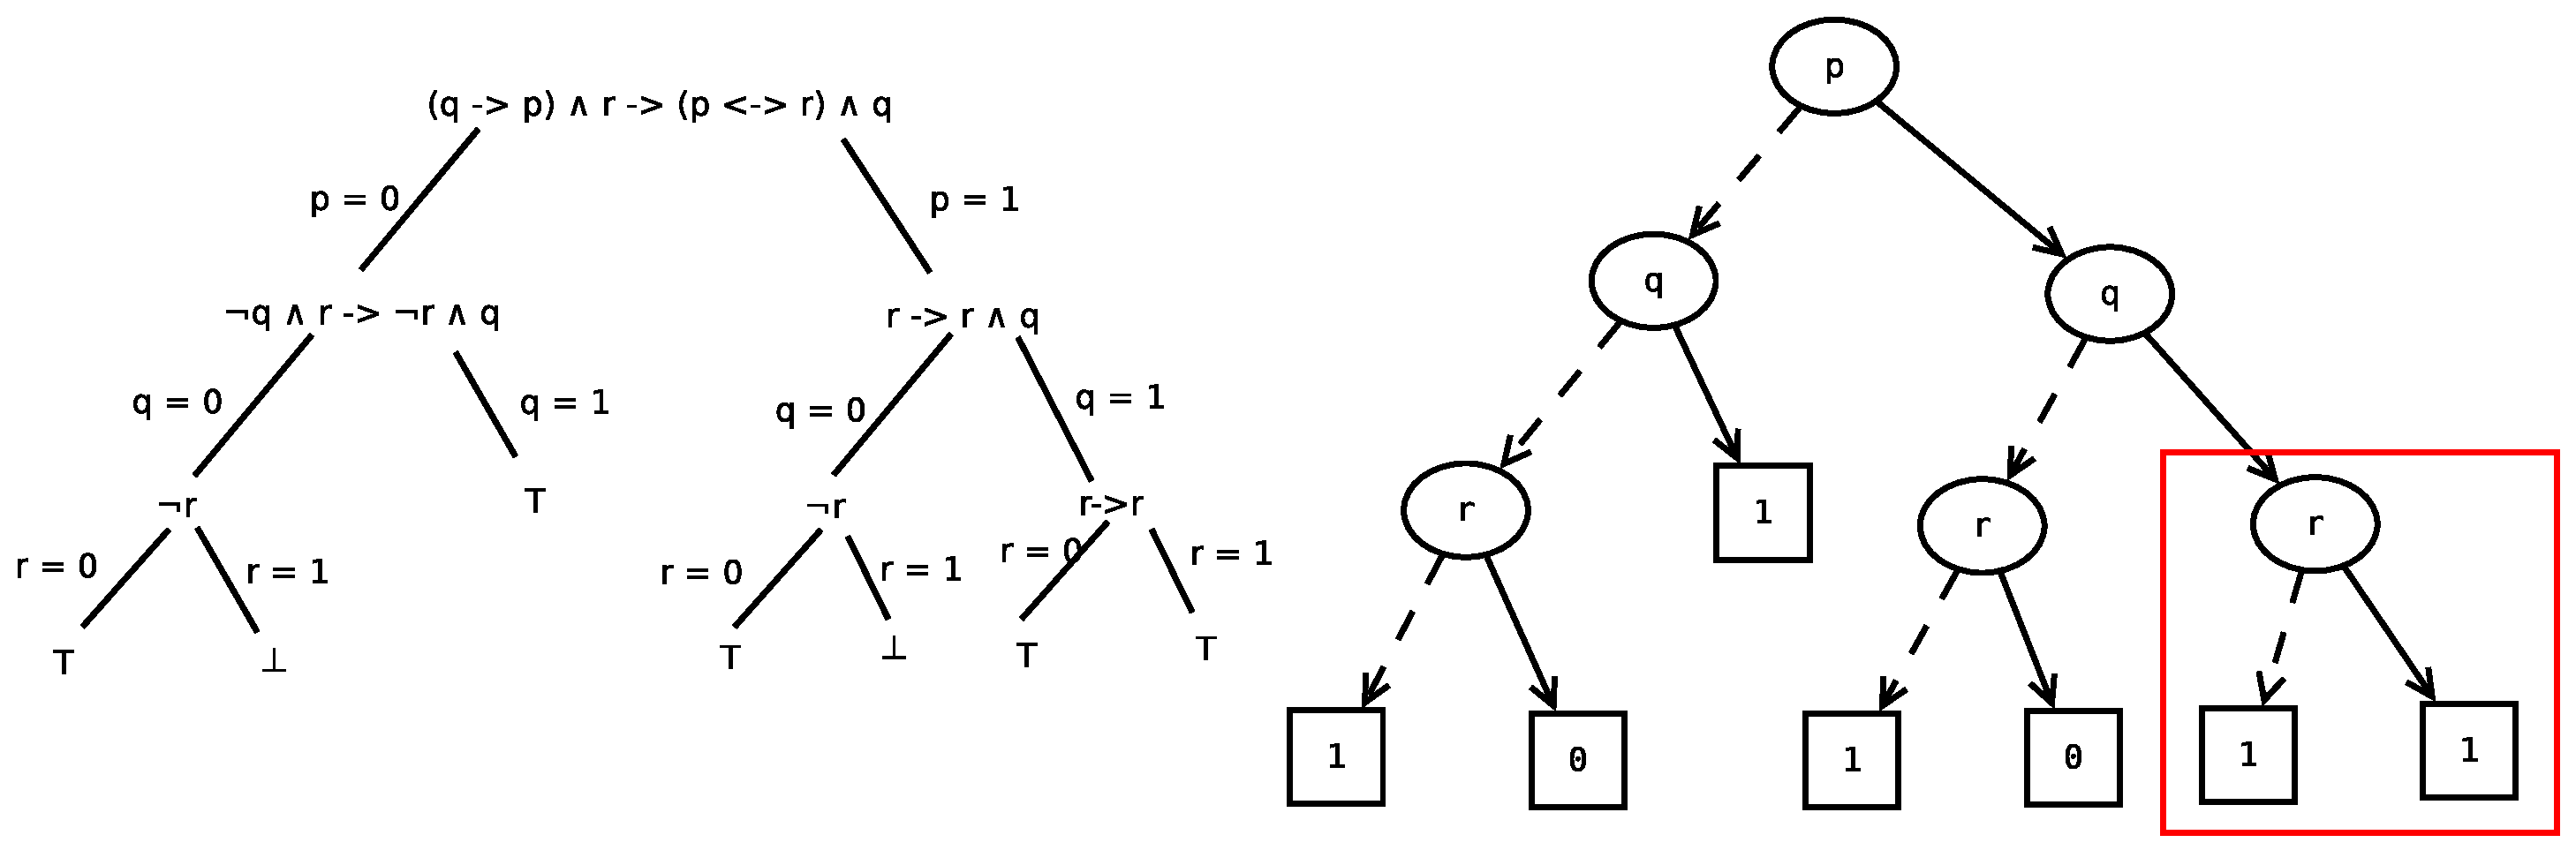
\includegraphics[width=1.25\textwidth]{SplittingToBinaryTree.eps}}

Note how this is formed from the splitting tree, insteadof formulas, we take a decision on a variable (with a circle) instead, with solid lines indicating a decision where the variable is true, and dashed lines indicating the variable is false. Also, in Binary Trees and OBDDs, we use 1 and 0 instead of $\top$ and $\bot$, and put a box around them. The red box is to indicate the first step we will take in making this an OBDD, and not part of the notation.

Now we will begin to convert this binary tree to an OBDD by removing isomorphic subtrees (which is where 2 subtrees are exactly the same as each other) and redundant tests (where a variable is tested, yet both its subtrees are exactly the same).

The first thing to note is that the bottom right r node (highlighted by the red box) had both branches leading to 1, meaning this test is redundant, we can remove it:

\centerline{\includegraphics[width=0.5\textwidth]{OBDDForming1.eps}}

The next thing to notice, is that now, both the subtrees leading from the p test are identical! This means we can get rid of half of this binary tree (the p test is now redundant), and only draw one of its branches, as they are both the same:

\centerline{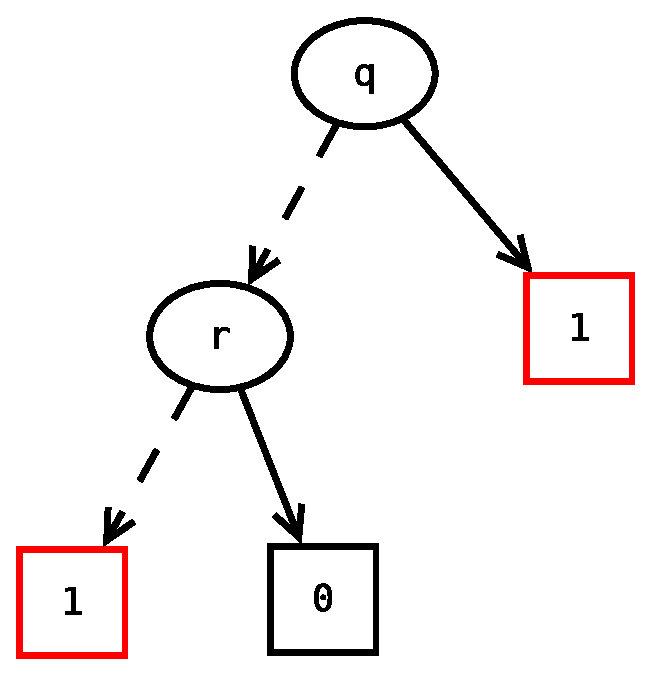
\includegraphics[width=0.25\textwidth]{OBDDForming2.eps}}

We're getting really close to an OBDD now! The last thing to note, is that there are multiple 1 nodes, this isn't allowed and so they must be rearranged:

\centerline{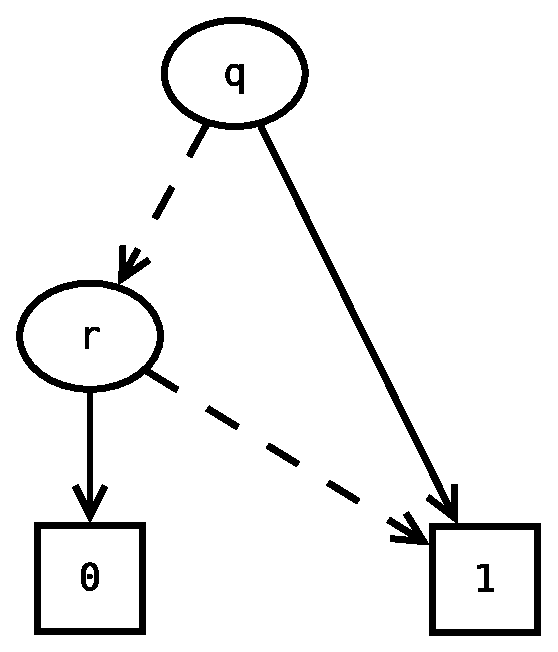
\includegraphics[width=0.25\textwidth]{OBDDForming3.eps}}

And there we have it! An OBDD! Note, we don't care what the original formula is, only the outcomes.

\section{Lecture 12}

Before we make an OBDD (ORDERED Binary Decision Diagram), we set an ordering for the decisions on the variables, to set the way the OBDD is formed, eg $p > q > r$.

This means that:
\begin{itemize}
\item Satisfiability checking can be done in constant time
\item Validity checking can be done in constant time
\item Equivalence checking can be done in constant time (because all the nodes are in the same order all the time now)
\item Boolean Operations are easy to implement.
\end{itemize}

The lecture slides show a good example of adding a formula to a binary dag, however, they do not clarify what they are actually showing!

The notes show a premade global dag, which is on the right, having the formula $(q \rightarrow p) \wedge r \rightarrow (p \leftrightarrow r) \wedge q$ merged into it. The example also uses the ordering $p > q > r$.

The algorithm recursively down the false side of the decision tree until it reaches 1/0, then begins returning, at which point it will go down the true side of nodes instead until it reaches 1/0. Before it returns a non 1/0 node, it will merge it into the existing global dag.

\section{Lecture 18}
Yes, I'm skipping a lot of lectures here, but I am moving onto everyone's favourite part of the course, LTL!

\subsection{Earlier bits of Lecture 18}

\subsection{LTL Basics}

LTL (Linear Temporal Logic) is a logic for reasoning about things with regards to time, particularly the future (but not the past).

Formulas in LTL are built in the same way as propositional logic, so anything that is a formula there will be a formula in LTL, there are some additions though:

If $F$ is a formula, then so is $\bigcirc F$, $\Box F$ and $\Diamond F$.

If $F$ and $G$ are formulas, then $F U G$ and $F R G$ are formulas. (Latex doesnt have the symbols for Until or Release, so I'm using U and R).

\vspace{5pt}
$\bigcirc$ is Next, this means in the next state, the formula will be true, so $\bigcirc F$ means in the next state that F will be true.

\vspace{5pt}
$\Box$ is always (in the future - it isn't applied retroactively), meaning that if a statement says $\Box F$, F will always be true.

\vspace{5pt}
$\Diamond$ is sometimes (in the future - again, not retroactive). So if we have $\Diamond F$, then in the future, F will be true at least once.

\vspace{5pt}
$U$ is until. So $F U G$ means that F will be true, until G occurs, and G must occur at a future position.

\vspace{5pt}
$R$ is release. $F R G$ means that F will be true, up to and including the state where G is true, if G never occurs, then F will be true forever. F can be any state after G occurs however.

\vspace{5pt}
If we have a series of states $\pi$ and $F$ which is an LTL formula, we can say that F holds on (is true on) the series of states, $\pi$, by saying
$\pi \models F$.

Any atomic formulas are true if they hold in $S_0$ of $\pi$.

Formulas on $\pi$ (taken straight from the notes):

\begin{enumerate}
\item $\pi \models \top$ and $\pi \not\models \bot$
\item $\pi \models X = V$ if $S_0 \models X = V$
\item $\pi \models F_1 \wedge ... \wedge F_n$ if for all $j = 1,...,n$, $\pi \models F_j$.
\\$\pi \models F_1 \vee ... \vee F_n$ if for some $j = 1,...,n$, $\pi \models F_j$.
\item $\pi \models \neg F$ if $\pi \not\models F$.
\item $\pi \models F \rightarrow G$ if either $\pi \not\models F$ or $\pi \models G$.
\\$\pi \models F \leftrightarrow G$ if either both $\pi \not\models F$ and $\pi \not\models G$ or both $\pi \models F$ and $\pi \models G$.
\item $\pi \models \bigcirc F$ if $\pi _1 \models F$
\\$\pi \models \Diamond F$ if at some state in $\pi$ we have $\pi _k \models F$.
\\$\pi \models \Box F$ if for all states, we have $\pi _i \models F$.
\item $\pi \models F U G$ if for some state, k, we have $\pi _k \models G$ and at all states before that, ($0$ to $k-1$), we have $\pi _j \models F$.
$\pi \models F R G$ if for all $K >= 0$, either $\pi _k \models G$ or, there is a value, $j<k$, so that $\pi _j \models F$.

\end{enumerate}

\section{Lecture 19}

\subsection{More LTL rules}

Two LTL formulas $F$ and $G$ are equivalent ($F \equiv G$), if for every path, $\pi$, we have $\pi \models F$ if and only if $\pi \models G$.

In LTL we can consider two kinds of properties:
\begin{enumerate}
\item Does $F$ hold on some computation path from an initial state?
\item Does $F$ hold on all computation paths from an initial state?
\end{enumerate}

Precedences of Connectives and Temporal Operators:

\begin{tabular}{l | r}
Connective & Precedence \\
\hline
$\neg$, $\bigcirc$, $\Diamond$, $\Box$ & 5 \\
$U$, $R$ & 4 \\
$\wedge$, $\vee$ & 3 \\
$\rightarrow$ & 2 \\
$\leftrightarrow$ & 1 \\
\end{tabular}
\end{document}
